%% LyX 2.3.4.2 created this file.  For more info, see http://www.lyx.org/.
%% Do not edit unless you really know what you are doing.
\documentclass[english]{article}
\usepackage[utf8]{inputenc}
\usepackage{amsmath}
\usepackage{hyperref}
\usepackage{amssymb}
\usepackage{graphicx}
\def\P{\mathbb{P}}

\makeatletter

%%%%%%%%%%%%%%%%%%%%%%%%%%%%%% LyX specific LaTeX commands.
%% Because html converters don't know tabularnewline
\providecommand{\tabularnewline}{\\}

\makeatother

\usepackage{babel}
\begin{document}
\title{Contribution of Schools to Covid-19 Pandemic: the Case of the Czech Republic}
\author{Martin \v Sm\'\i d, Jakub Drbohlav, Milan Zaj\'\i\v{c}ek\thanks{Institute of Information Theory and Automation of the CAS, BISOP}}
\maketitle

\section*{Main findings}
\begin{itemize}
\item In-person education is a significant source of infections in the children age cohorts, yet the majority of those infections come for other sources than schools
\item Data suggest negligible or zero effect of children attendance to kindergartens
\item The effect increases with the age and is significantly higher in secondary schools
\item The effect of particular opening regimes can be evaluated. For instance, opening of the first degree of primary schools increases weekly infections in the cohort approximately by $41\%$, the analogous value for secondary schools is $47\%$.

%\item The effect of ordering masks in classrooms is significant

\item Data do not support the hypothesis that closing schools causes additional infections in other environments

\item A simple indicator of safe opening of schools may be constructed. Using it, we can conclude that closing schools in Czechia during the school year 20/21 was mostly reasonable given the state of surrounding epidemics; however, the spring opening of primary schools could have been quicker
\end{itemize}

\section*{Introduction}

Closing schools during the present pandemics is the one of the most
controversial issues. According to epidemiological mainstream, schools
are strong drivers of respiratory diseases \cite{gold_clusters_2021,stein-zamir_large_2020,torres_severe_2020}; see also 
\cite{forbes_association_2021,sage_tfc_nodate, ismail_sars-cov-2_2021, lessler_household_2021, brauner_inferring_2021,haug_ranking_2020}, but also 
\cite{zhu_meta-analysis_2020, zimmerman_incidence_2021}; therefore, closing
schools was one of the first governmental reactions to the outburst
of the present pandemic. However, the price the society pays for closing schools
is high. Online education is not an equivalent substitute for the
in-person one \cite{dipietro_impact_2020, engzell_learning_2020, maldonado_effect_nodate}; moreover, the isolation of students leaves deficits
in their necessary social contacts \cite{bignardi_longitudinal_2020,
noauthor_covid-19_2020,dipietro_impact_2020,ravens-sieberer_impact_2021}. Thus, for the society,
decision whether and when to close schools means a painful trade-off,
making any decision political rather then scientific; science, however,
has irreplaceable role in giving the best possible (quantitative)
basis for these decisions. 

Unfortunately, it is difficult to evaluate the effect of closing schools
in the context of the current pandemic. The virus was completely unexplored as
it came and its knowledge increased only gradually, so we only gradually
get to know whether and how differently the virus affects children
in comparison with the rest of the population. To estimate the effect
from running epidemic data is also problematic, mainly because the
counter-epidemic measures are usually being introduced (and released)
together, so it is difficult to distinguish their effects, and even
in cases when the measures are applied in different times, still they
can be assessed only in the context of the other measures applied.
\cite{brauner2021inferring}, for instance, regards school closure as a very
effective means of curbing the present pandemics; however, it is necessary
to take into account that school closures were usually the first measures
applied, so their measured effect may be overestimated in comparison with the other measures.

In our analysis, we exploit a ``gap'' in this puzzle: the fact that
certain age cohorts of children nearly uniquely correspond to the
degrees of schools and, except for kindergartens, the vast majority of
children do attend their classes. Thus it could be expected that
closing (opening) of particular degrees will result in significant
changes in infections in the corresponding cohorts. The other measures,
on the other hand, are usually much less age specific (wearing masks,
bans of gatherings, for instance) or are affecting different age cohorts (home office)
so they can be expected not to obscure much the effects of school closures.

To evaluate the effects of the closures, we used a simple epidemiological-like
model, in which the infections in the children cohorts in each district depend on the
overall magnitude of epidemic, its magnitude within the district and within the corresponding cohort, the latter in dependence on the current school opening regime. Using our model, we estimate quantitative impact of various regimes of school opening to the infections within the corresponding cohort.
Next we construct a simple estimator of the infection grow within the cohort, which can be useful for for decisions on school restriction degree during the epidemic. and we apply it retrospectively to the school year 2020/21.

We estimate our model by means of the data from the covid-19 pandemic in the Czech Republic. Here, all the primary and the secondary schools
had been closed on March 12, 2020, shortly after the first cases of
covid infection appeared. The schools were opened in May only in a very limited
regime until the summer vacation. After the vacation, all the schools
had been opened for two weeks nearly without any restriction. Next,
after the overall infection numbers started to rise, wearing masks in classrooms
had been imposed. In the end of October, after the serious increase of
infections, all the schools had been closed until except
for kindergartens, which remained open until February 27, 2021. Following a partial amelioration, schools started to be gradually opened. During the last weeks before Christmas, first degree, the last year of the second degree and the last year of the secondary schools had been fully opened (with masks), while the remaining years (6th to 8th) of the second degree had been opened in weekly rotation regime. After the Christmas holiday, however, all schools had been closed again except for the  first two years of the first degree and the kindergartens, which all remained open until February 27. On April 12th, 2021, kindergartens were opened for the final year and the first degree was open in the rotation regime with testing in schools. In the following weeks, all the schools had been gradually opened, usually starting with the rotation regime, following by the full regime with masks, later without masks in classroom, all with regular testing at schools except for kindergartens. See Table \ref{tab:measures} for the detailed schedule.

%https://www.idnes.cz/zpravy/domaci/skoly-navrat-deti-studenti-zakladni-skola-andrej-babis-koronavirus-epidemie.A201111_091753_domaci_rapc

%https://www.irozhlas.cz/zpravy-domov/koronavirus-online-v-cesku-cesko-cr-navrat-do-skol-skolstvi-robert-plaga-jan_2011191400_ako
\begin{table}
\begin{center}
\small
\begin{tabular}{l|c|c|c|c}
Date	&	Kindergartens		&	First degree	&	Second degree	&	Secondary \\
\hline
Mar-13	& volantury	& \multicolumn{3}{c}{closed}\\
May-04	&			&		&	&	\\
May-11	& & &  \multicolumn{2}{c}{last year max. 15 voluntary} \\
May-25    &  & max. 15 voluntary & &  \\
Jun-08	& &  & \\
Jun-26	&	\multicolumn{4}{c}{end of the school year} \\
Sep-01	&	\multicolumn{4}{c}{start of the school year, opened} \\
Sep-17	&	  & \multicolumn{3}{c}{masks ordered in classrooms} \\
Oct-05	&  & & & some closed \\
Oct-14	&  & \multicolumn{3}{c}{closed} \\
Nov-18	&  &  $1^{st}$ $2^{nd}$ open &  &  \\
Nov-25	&  &  & & last year open \\
Nov-30  & & open & rotations, last yr. open & \\
Jan-04	&  & $1^{st}$ $2^{nd}$ open &  closed & closed \\
Feb-27	&    \multicolumn{2}{c}{closed}  & \, & \\
Apr-12  & last years & rotations & &  \\
Apr-26  &  selected open & & &  \\
May-03  &  & & selected rotations &  \\
May-10  & open & & rotations & \\
May-17  & & open with testing & selected open w. t. & \\
May-24 & & & open with testing & open with testing \\
Jun-08 &  & \multicolumn{3}{c}{masks not required in all but 3 regions} \\
Jun-15 &  & \multicolumn{3}{c}{masks not required} \\
June-30 & \multicolumn{4}{c}{end of school year}
\end{tabular}
\caption{Schedule of counter-epidemic measures at schools in 3/2020-6/2021.}
\label{tab:measures}
\end{center}
\end{table}


\section*{Methods}

To determine the influence of attending schools of a given kind, we examine the number of reported infections $X_{i,t}$ in the corresponding age cohort for each district $i$ at time $t$. Generally, we assume that this number depends on the previous-week number of infections, the contact restriction reported two weeks earlier, and current rate of infectiousness. In addition to the total number of infections in population, we take into account the number of infections in the same district, and the number of infections in the same cohort within the district. See Appendix \ref{sec:epimodel} for the justification of this general model. We also consider the influence of school opening regime on the infection number in the cohort. In particular,
\begin{equation}
X_{i,t} = \alpha_i D_t Y_{t-1} + \beta_i D_t Y_{i,t-1} + \gamma D_t X_{i,t-1}
+ S_t X_{i,t-1} + e_{i,t}
\label{eq:x}
\end{equation}
$$
D_t = d_t C_{t-2},\qquad
S_t = D_t (\nu N_{t-1} + \mu M_{t-1} + \varrho R_{t-1} + \nu^\star N^\star_{t-1}
+ \mu^\star M^{\star}_{t-1} + \varrho^\star R^\star_{t-1} 
)
$$
for each district $i$ and time $t$. Here, $Y_t$ is the number of overall infections within the population at $t$, $Y_{i,t}$ is the number of infections within the $i$-th district at $t$, $N_t$, $M_t$, $R_t$ evaluate the degree of school opening without masks, with masks, with weekly rotations (with masks on), respectively (zero means all classes closed, one means all classes opened), $N^\star_t$, $M^\star_t$, $R^\star_t$ stand for the same regimes with the addition that students are regularly tested at schools,  and $e_{i,t}$ is the error term. Finally, $d_t$ is the (predicted) rate of infectiousness and $C_t$ is the contact restriction at $t$, see Appendix \ref{sec:epimodel} for details.

We estimate the impact of school opening four ways: by comparing two sub-cohorts of the examined cohort assuming each of them to follow (\ref{eq:x}) either with the same or with different school regime coefficients $\nu,\mu,\dots,\varrho^\star$, by estimating parameters from (\ref{eq:x}) applied to the whole cohort and, finally, by estimating the parameters from simplified version of (\ref{eq:x}) with homogeneous impact of districts.

{\em Comparison of two sub-cohorts with different regime parameters (later abbreviated as S).} Here we consider two sub-cohorts of comparable size, the $j$-th one following its own version of (\ref{eq:x}):
$$
X^j_{i,t} = \alpha^j_i D_t Y_{t-1} + \beta^j_i D_t Y_{i,t-1} + \gamma^j c_j D_t X_{i,t-1}
+ S^j_t c_j X_{i,t-1} + e^j_{i,t}
$$
$$
S^j_t = d_t [\nu^j N^j_{t-1} + \mu^j M^j_{t-1} + \varrho^j R^j_{t-1} + \mu^{\star j} M^{\star  j}_{t-1} + \nu^{\star j} N^{\star j}_{t-1} +  \varrho^{\star j} R^{\star j}_{t-1} ],
$$
where $c_j$ is the relative size of the $j$-th sub-cohort with respect to whole cohort. By subtracting, we get 
\begin{equation}
\frac{X^{1}_{i,t}}{c_{1}} - \frac{X^{2}_{i,t}}{c_{2}} = \alpha'_i D_t Y_{t-1} + \beta'_i D_t Y_{i,t-1} 
+ \gamma' D_t X_{i,t-1} + U_t X_{i,t-1} + e'_{i,j,t}, \qquad U_t = S^1_t - S^2_t.
\label{eq:dif}
\end{equation}
Clearly, for the regime coefficients pairs $(\nu^1,\nu^2),\dots,(\varrho^{\star 1},\varrho^{\star 2})$ to be estimable, the corresponding covariate pairs $(N^1,N^2),\dots,(R^{\star 1},R^{\star 2})$ have to differ sufficiently. In the case or kindergartens, for instance, the only regimes having been applied were opening without masks ($N^1_t = N^2_t = 1$), opening only for the last years ($N^1_t=1,N^2_t=0$) and closure ($N^1_t = N^2_t = 0$), which is enough for $\nu^1$ and $\nu^2$ to be estimable. Yet only a minority of coefficients happened to be estimable this way, the clear advantage here is that the covariates and coefficients which do not differ cancel out, so our estimate is independent both of these parameters and on the choice of corresponding regime covariates, which are set subjectively sometimes, for instance when the only a subset of classes is opened. Moreover, even though we do not explicitly assume the same impact of the external environment on both the sub-cohorts, these impacts are likely to be are similar, so they more or less compensate by the subtractions. Note also that the results of this estimation can also be used to test the null hypothesis that the corresponding regime has no influence on infections, which will be rejected by significant values of either $\nu^{1}$ or $\nu^2$.\footnote{The significance level has to be corrected here.} 

{\em Comparison of two sub-cohorts with common regime parameters (SC).} If we decrease the generality of (\ref{eq:dif}) by assuming that $\nu^1 = \nu^2 = \nu$, $\dots$, $\varrho^{\star 1} = \varrho^{\star 2} = \varrho^{\star}$, we get
$$
U_t = d_t [\nu \Delta N_{t-1} + \dots + \varrho^\star \Delta R^\star_{t-1}  ] 
\qquad \Delta N_{t}= N^1_{t}-N^2_{t},\dots,
\Delta R^\star_t = R^{\star 1}_{t}-R^{\star 2}_{t´}
$$
from which we can estimate those of the regime coefficients  for which the corresponding covariates differ at least for some time. Again, the significant values may serve for the proof that the opening in the particular regime influences infections.

{\em Estimation from (\ref{eq:x}) for the whole cohort (W).} For the coefficients corresponding to the regimes which had never differed between the sub-cohorts, there is nothing to do but to estimate them directly from (\ref{eq:x}). 

{\em Estimation from a homogeneous version of (\ref{eq:x}) (WH).} Finally, to get global results rather than the district-level ones, we decrease the generality of (\ref{eq:x}) and assume a homogeneous model:
\begin{equation}
X_{i,t} = \alpha h s_i D_t Y_{t-1} + \beta h D_t Y_{i,t-1} + \gamma D_t X_{i,t-1}
+ S_t X_{i,t-1} + \epsilon_{i,t}.
\label{eq:linear}
\end{equation}
Here, $h$ is the relative size of the examined cohort with respect to the rest of the population and $s_i$ is the relative size of the $i$-th district's population.
By summing (\ref{eq:linear}) over $i$, we get 
\begin{equation}
X_{t} =  \omega h D_t Y_{t-1}
+ (\gamma D_t +  S_{t})X_{t-1} + \epsilon_{t}, \qquad \omega = \alpha +\beta,
\label{eq:xss}
\end{equation}
where $X_t$ is number the overall cohort infections, which may be alternatively interpreted as
\begin{multline}
\P[\text{infection in cohort at $t$}]
\\
\doteq \omega D_t  \P[\text{overall infection at $t-1$}] + (\gamma D_t +  S_{t}) \P[\text{infection in cohort at $t-1$}]
\label{eq:p1}
\end{multline}
(to see it, divide (\ref{eq:xss}) by the cohort size). 
Similarly, we can interpret 
(\ref{eq:linear}) as
\begin{multline}
\P[\text{infection in the cohort in district $i$ at $t$}]
\\
\doteq \alpha s_i D_t \P[\text{overall infection at $t-1$}]
+\beta D_t \P[\text{infection in district $i$ at $t-1$}] \\
+(\gamma D_t + S_{t}) \P[\text{infection in the cohort in $i$ at $t-1$}]
\label{eq:p2}
\end{multline}
(again, it suffices to divide (\ref{eq:linear}) by the cohort size). It is clear from (\ref{eq:p1}) and (\ref{eq:p2}) that quantities $\alpha D_t$, $\beta D_t$, $\gamma D_t$, $\nu d_t, \dots, \varrho^\star d_t$ may be seen as weights, contributing to the infection in the cohort in the hypothetical case that the probability of infection is the same in the population, in the district and in the cohort.
\def\defined{\stackrel{\text{def}}{=}}

Finally, if we divide (\ref{eq:xss}) by $X_{t-1}$, we get the relative growth of infections within the cohort:
\begin{equation}
\rho_t \defined {\mathbb E} \left(\frac{X_{t}}{X_{t-1}}|\text{history up to $t-1$}\right)=G_t + S_t
\qquad G_t = D_t \left[\omega \frac{h Y_{t-1}}{X_{t-1}}+\gamma \right],
\label{eq:rhodef}
\end{equation}
from which we can distinguish the part of the growth caused by school opening (quantified by $S_t$) from that originated outside schools ($G_t$). In the special case that no contact restriction is applied ($D_t=d_t$) and that the ratio of infected in the cohort is the same in as that within the whole population (i.e. $\frac{h Y_{t-1}}{X_{t-1}}=1$) we get
\begin{equation}
\rho_t = d_t (\omega + \delta + \nu N_{t-1} + \dots + \varrho^\star R^{\star}_{t-1})
\label{eq:rhoproc}
\end{equation}
i.e. the regime coefficients themselves may serve as weights.


\section*{Data}

In the Czech Republic, each September first, children who completed
their sixth year are obliged to enter the first grade of an elementary
school. When the parents wish, a child who is six as late as by the
end of the year can enter the first class, too, some children, on
the other hand, start their school later for various, mostly developmental,
reasons. If we neglect these exceptions, we can conclude that the
first year pupils are six or seven; consequently the vast majority of the first degree 
(first five grades) pupils belong to the age cohort $6-11$, the vast majority of the  second
degree (the sixth to the ninth year) students belong to the cohort $11-15$, and 
the students of secondary schools, which typically take four
years in the Czech Republic, belong to the cohort $15-19$. As for the kindergartens, where the lowest
age for admission is three, the vast majority
of children attending kindergartens falls into the cohort $3-6$.

For simplicity we assume that the frontier one-year cohorts split
by half between the competing school categories, so the infections
happening in the cohort split by two between each category. 
Consequently, the number of cases by pre-school children over week $t$ in
the $i$-th district will be $X_{i,t}^{k}=Z_{i,t}^{3}+Z_{i,t}^{4}+Z_{i,t}^{5}+\frac{1}{2}Z_{i,t}^{6}$,
the number by the first degree $X_{i,t}^{f}=\frac{1}{2}Z_{i,t}^{6}+Z_{i,t}^{7}+\dots+\frac{1}{2}Z_{i,t}^{11}$,
by the second degree $X_{i,t}^{s}=\frac{1}{2}Z_{i,t}^{11}+Z_{i,t}^{12}+\dots+\frac{1}{2}Z_{i,t}^{15}$
and that by the secondary schools $X_{i,t}^{e}=\frac{1}{2}Z_{i,t}^{15}+Z_{i,t}^{16}+\dots+\frac{1}{2}Z_{i,t}^{19},$where
$Z_{i,t}^{j}$ is the number of cases by the $j$-year old individuals
in the $i$-th district. 
We take the values $Z^j_{i,t}$ from the public dataset by the Czech Ministry of
Health, namely the anonymized person-level list of reported infections
(cit osoby.htm) including, among other things, the date of reporting
the infection and the age; the series $Y_t$ and $Y_{i,t}$ are computed by their aggregation.

Yet the first cases in Czechia appeared in the beginning of March, 2020, we do not take data until April 5th, 2020 into
account, as we regard them as noisy, unreliable
and suffering from small sample properties. The last values used for the estimation correspond to the week staring on June 28th, 2021. As we do not use data from 9 weeks of summer vacation and those from the one-week Christmas vacations, this means 53 weeks. As there is 77 districts (including the capital), this gives 4081 observations, from which, however, some additional ones were excluded, see below.

The regime covariates have been determined according to measures schedule, listed in Table \ref{tab:measures}. The values of $N,\dots,R^\star$, which correspond to the full cohorts, were set to $1$ if the corresponding regime applied fully, and to $0$ if it was not applied at all given week, some values were set to fractional values. Some of these observations were excluded from estimation of (\ref{eq:x}) and (\ref{eq:dif}), especially in the cases when the fractional value could not be determined objectively. We also excluded observations corresponding to holidays and the weeks with no more than two possible school days, as our study concerns only weeks in which the teaching takes place, perhaps online. The list of values of the regime covariates can be seen in Table TBD
in Appendix together with the notes on how we determined fractional
values and reasons of observation exclusions. 

We identified four opportunities for sub-cohort comparison. The first were two weeks starting from April 12th when the kindergartens have been open only for the last (pre-school) year, the second when only the first two years out of the first degree were open in January and February 2021, the third when the second degrees were open for the last year while the rotation regime was applied for the rest starting from November 30th, 2020 until Christmas vacation, the fourth when only the last year of secondary schools were open from November 25 until the Christmas vacation. As control groups, we chose the closest year (or years) for which their corresponding sub-cohorts do not share a border cohort. For kindergartens, where the percentage attending them decreases with the age, we chose four year old as the control sub-cohort, because it is closer to the treatment group. The details on the sub-cohort models are summarized in Table \ref{tab:sc}. For the values of the covariates, see Appendix TBD.

\begin{table}
\begin{center}
\begin{tabular}{l|cccc}
& Kindergartens & First degree & Second degree & Secondary  \\ \hline
Group 1 & last year & 1st and 2nd yr. & 9th year & 4th year \\
Sub-cohort 1 & $\frac{1}2 (Z^5 + Z^6)$ & $\frac{1}2 Z^6 + Z^7 + \frac{1}2 Z^8$  
& $\frac{1}2 (Z^{14} + Z^{15})$ &  $\frac{1}2 (Z^{19} + Z^{20})$ \\ \hline
Group 2& 5 year old & 4th and 5th yr. & 7th year  & 2nd year  \\
Sub-cohort 2 & $Z^4$ &
$\frac{1}2 Z^9 + Z^{10} + \frac{1}2 Z^{11}$  
& $\frac{1}2 (Z^{12} + Z^{13})$ &  $\frac{1}2 (Z^{17} + Z^{18})$ 
\\ \hline
Period & 4/12 -- 4/25/21 & 1/4 -- 2/16/21 & 11/30 -- 12/21/20 & 11/25 -- 12/21/20 \\
Full weeks & 2 & 8 & 3 & 3 \\ \hline
Diff. pars. & $\nu^1,\nu^2$ & $\mu^1,\mu^2$ & $\mu^1,\rho^2$ & $\mu^1,\mu^2$ \\ 
Common pars. &  & $\mu$ & $\mu-\rho$ & $\mu$ \\ 
\end{tabular}
\caption{Details on sub-cohort comparisons}
\label{tab:sc}
\end{center}
\end{table}





\section*{Results}

We estimated all S, SC, W and WH by weighted least squares where we took 
$
w_{i,t}=\max(20^2, Y^2_{i,t-1})
$ as weights of residual variances. This choice was motivated by residual analysis and our desire to suppress observations suffering from the small-sample property.  The detailed results of the estimation may be found in Table \ref{tab:params} (Appendix) and seen in Figure  
\ref{fig:comp} (recall that the regime coefficients always evaluate the rate of infections caused by the own cohort up to $d_t$, so they are comparable each with other as well as between the cohorts).
\begin{figure}
\begin{center}
\begin{tabular}{ccc}
First degree & Second degree & Secondary \\
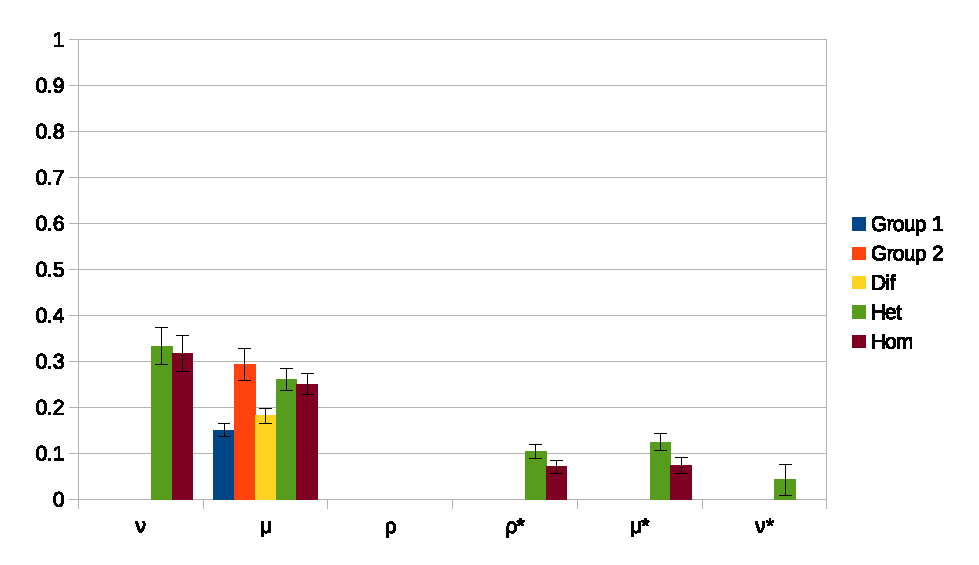
\includegraphics[width=4cm]{fdcoef.eps} 
&
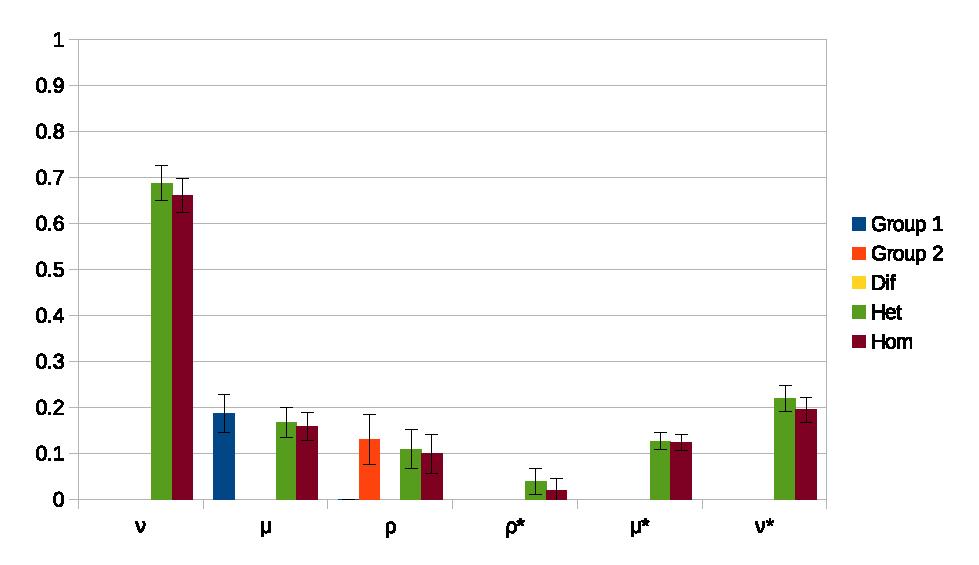
\includegraphics[width=4cm]{sdcoef.eps} 
&
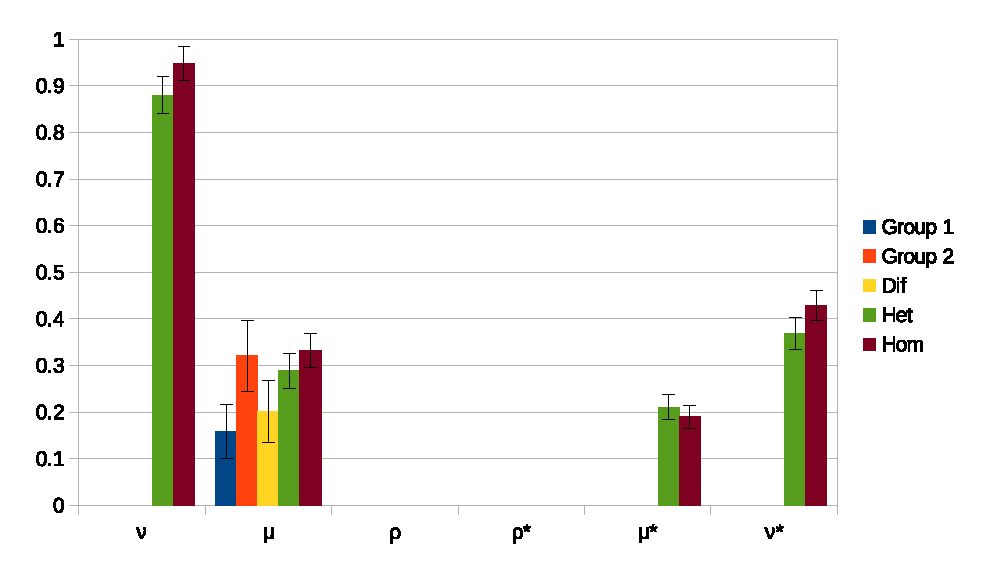
\includegraphics[width=4cm]{seccoef.eps} 
\end{tabular}
\caption{Comparison of regime coefficients}
\label{fig:comp}
\end{center}
\end{figure}

Further, we computed aggregated estimates of the regime parameters as the weighted average of the estimates by the individual models, where we gave weight $55\%$ to model DC (which we regard as most independent of exogenous influences), $15\%$ to each of the two estimates given by D, $10\%$ to W and $5 \%$ to WH. The results may be found in Table \ref{tab:metacomp} together with the percentage increase of the growth given no contact restriction (see (\ref{eq:rhoproc})) and tge reliability of the estimate, which we evaluate as the sum of weights of source estimates at our disposal. 

\begin{table}
\begin{center}
\small
\begin{tabular}{l|ccc|ccc|ccc} Para- & \multicolumn{3}{c}{First degree} & \multicolumn{3}{c}{Second degree} & \multicolumn{3}{c}{Secondary} \\ meter  & par. & inc. & rel. & par. & inc.& rel.& par.& inc. & rel.\\  \hline  
$\nu$& $0.33(0.04)$& $0.66$&$0.15$& $0.68(0.04)$& $1.04$&$0.15$& $0.9(0.04)$& $1.91$& $0.15$\\
$\mu$& $0.21(0.02)$& $0.42$&$1$& $0.18(0.04)$& $0.27$&$0.3$& $0.23(0.06)$& $0.48$& $1$\\
$\rho$&&&& $0.12(0.05)$& $0.18$&$0.3$&&& \\
$\rho^\star$& $0.09(0.02)$& $0.19$&$0.15$& $0.03(0.03)$& $0.05$&$0.15$&&& \\
$\mu^\star$& $0.1(0.02)$& $0.2$&$0.15$& $0.13(0.02)$& $0.19$&$0.15$& $0.2(0.03)$& $0.43$& $0.15$\\
$\nu^\star$& $0.08(0.03)$& $0.17$&$0.15$& $0.21(0.03)$& $0.32$&$0.15$& $0.39(0.03)$& $0.82$& $0.15$\\
$\gamma$& $-0.05(0.03)$& –& –& $-0.09(0.03)$& –& –& $-0.17(0.03)$& –& –\\
$\omega$& $0.55(0.04)$& –& –& $0.74(0.06)$& –& –& $0.65(0.06)$& –& –\\
\end{tabular}

\caption{Aggregated estimates of regime coefficients.{\em par.} -- aggregated estimate(standard error), {\em inc.} -- percentage increase given no contact restriction (see (\ref{eq:rhoproc})), {\em rel.} -- the sum of source coefficients' weights.}
\label{tab:metacomp}
\end{center}
\end{table}

\begin{figure}
\begin{center}
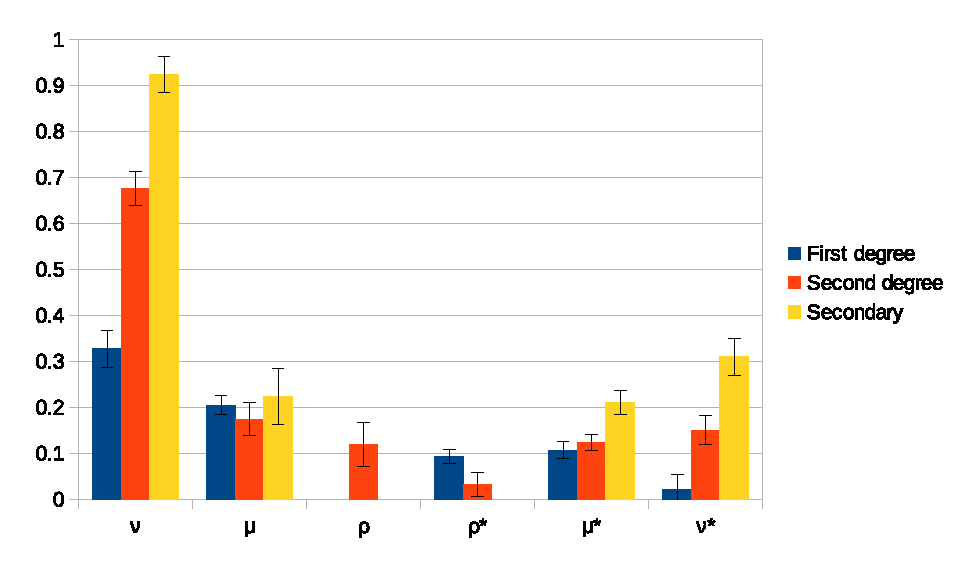
\includegraphics[width=7cm]{coefs.eps}
\caption{Comparison of meta-estimated regime coefficients}
\label{fig:metacomp}
\end{center}
\end{figure}

Next, for each cohort with the exception of kindergartens. we evaluated the predictions of the growth rate $\rho_t$ and compared them with actual values. For the predictions, we used the aggregated parameters (Table \ref{tab:metacomp}). The results are depicted in Figure \ref{fig:rho}. where the value $\rho_t$ is also decomposed into individual parts, i.e. $G_t$ and the components of $S_t$ corresponding to individual regimes

\begin{figure}
\begin{tabular}{ccc}
First degree & Second degree & Secondary \\
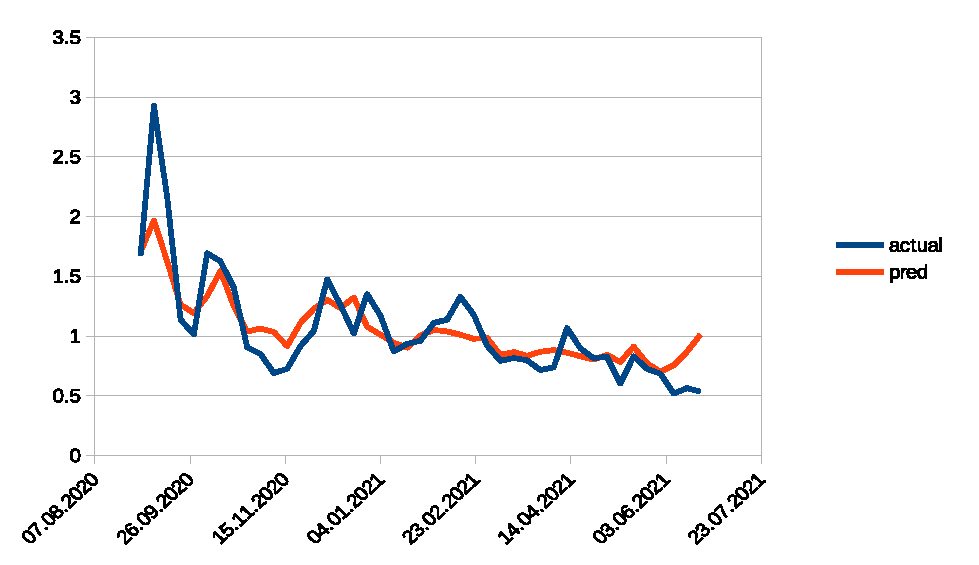
\includegraphics[width=4cm]{rhofa.eps} &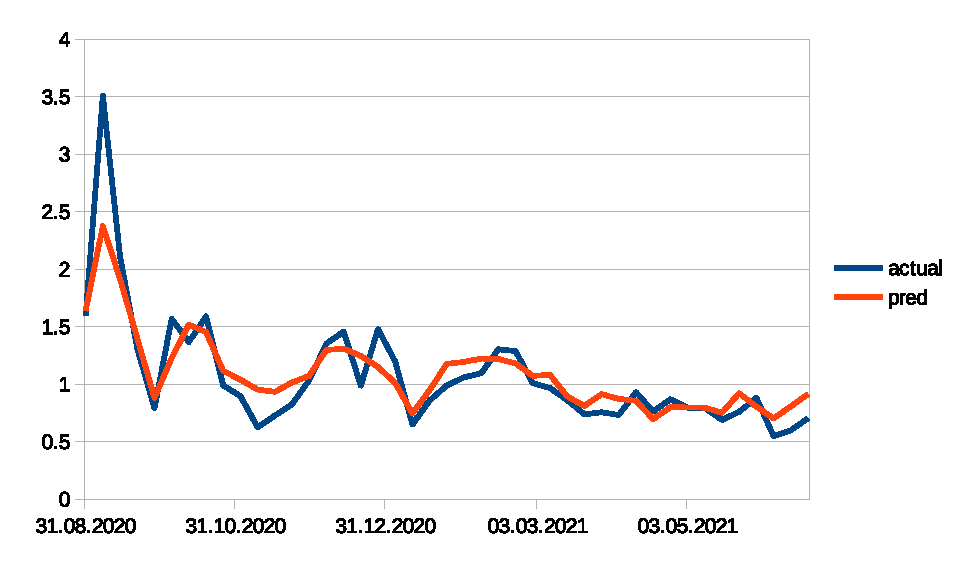
\includegraphics[width=4cm]{rhosa.eps}&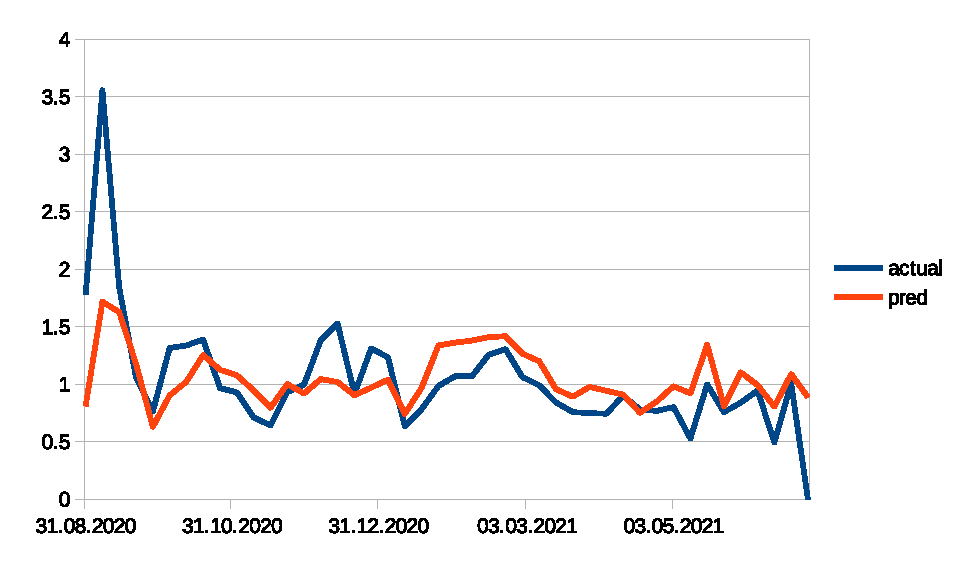
\includegraphics[width=4cm]{rhoseca.eps} \\
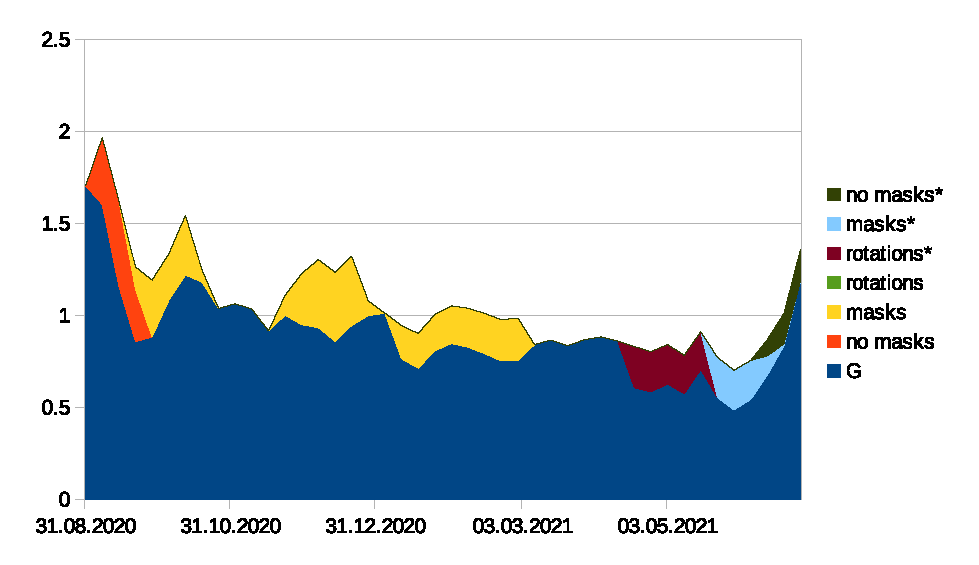
\includegraphics[width=4cm]{rhof.eps} &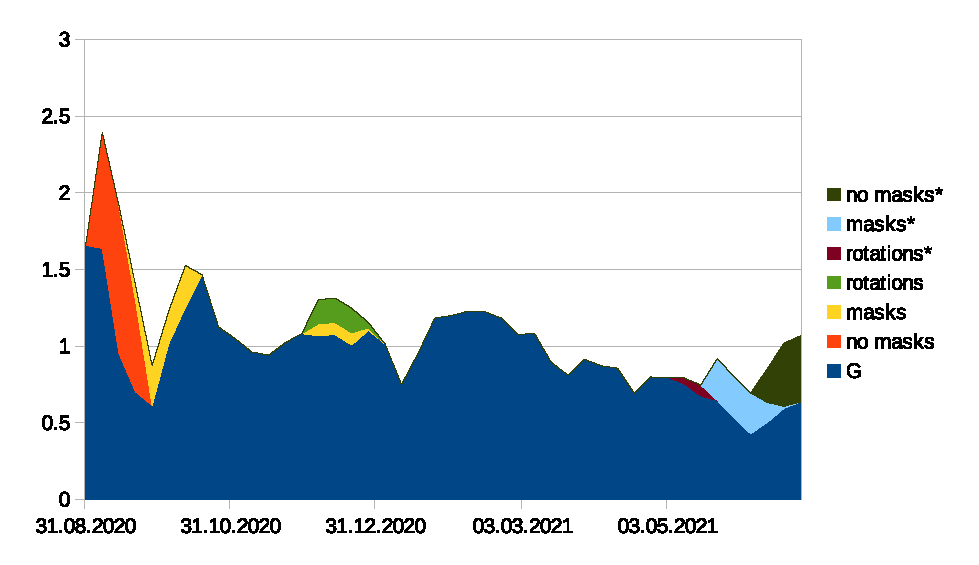
\includegraphics[width=4cm]{rhos.eps}&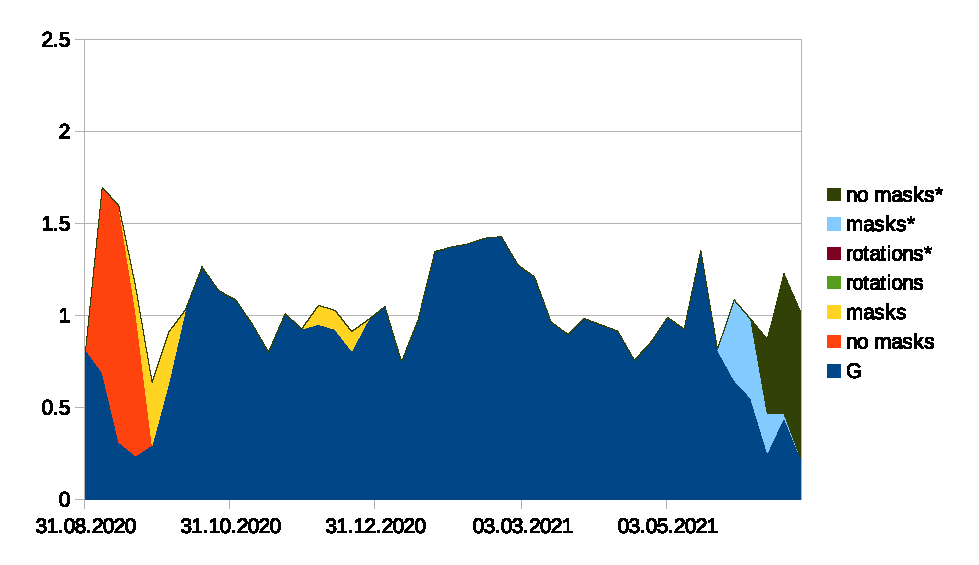
\includegraphics[width=4cm]{rhosec.eps} \\
\end{tabular}
\caption{Increases in cohort ($X_{t}/X_{t-1})$, $\rho_t$ and its decomposition. TBD: into same graphs!}
\label{fig:rho}
\end{figure}





\section*{Discussion}

The presented results chart a consistent picture of the relations between school opening and infections. Almost beyond doubt we demonstrated that opening of primary as well as secondary schools does have a significant  influence on the infections within corresponding age cohorts of students. Kindergartens, on the other hand, appear to have negligible or no impact. Our results also demonstrate that the influence grows with the age of students. We are also able to quantify the influence of various regimes, especially for the case of mandatory wearing masks in classrooms, which we were able to estimate reliably by means of sub-cohort comparison. 

The main limitation of our study is the possible dependence on time, hence on specific temporal circumstances. Even in the case of the most environment-independent method -- evaluating differences between sub-cohorts (D and DC) -- as the measures are applied statewide, all the observations with the positive difference between covariates come from a time period which is an exclusively different from that from which the observations with zero differences come. Usual technique of adding time dummies thus cannot be applied here is the dummies would be co-linear with the alleged difference. On the other hand, the fact that the estimates of the regime coefficients coming from different models, some of which use maximum number of observations over time, do not differ significantly, speaks in favour of their validity. 

The results are also sensitive to the choice of the infectiousness rate $d_t$, which we estimated from the  global history of the epidemics, regardless the age, see Appendix TBD. As no children younger than 16 were vaccinated by June 2021 and only a small minority of students over 16 had got their first dose by that time, we did not include the effect of vaccination in $d_t$. We also did not include possible effect of immunization. However, once it is included by assuming that the number of immune individuals in the children cohort is equal to the number of reported cases so far and $d_t$ is multiplied accordingly, the estimation gains quite similar results, see Appendix \ref{sa:im}.

Another issue to be considered is that the number of reported infections is less than the number of actual infections. This would not be problem if the ratio of reported to infected did not change over time. If the ratio were constant and the same for all the age cohorts, then our models, lacking a constant term and hence being linear, would hold with the same coefficients for the reported values as they would for the actual ones; if the ratio were constant but differing between the examined cohort and the overall population, then the bodel would hold too, but with different coefficients. However, this issue makes a problem when the ratios change over time. The probelm is less if they change gradually and accordingly between cohorts (then only the small changes between weeks would matter), but the problem would be serious if, for instance, the ratio jumps for the students but not for the rest of the population, as it is the case when testing is introduced tu schools. As a result, the starred coefficients (regimes including testing at schools) will likely be overestimated and we should be cautious when comparing them with the non-starred ones. Another probable change of detection ratio happened in the beginning of September 2020, when a recommendation (cit %https://koronavirus.mzcr.cz/wp-content/uploads/2020/09/Metodick%C3%BD-postup_OSPDL_MZ_Covid-ve-%C5%A1kol%C3%A1ch.pdf?fbclid=IwAR193MQUjdD06dm9AhJTl3W60gQfJFdDJFDfpDhjX_KtJ6KAwvjOMCT1WzE
) has been issued not to test children exhibiting symptoms; it is likely that this issue stands beyond the jumps in Figure \ref{fig:rho} in September.
%; however, the recommendation ceased to hold (TBD when?) so it influenced only a minority of observations. 

Further, there is a determinant of children infections not taken into
account in our analysis: encounters with teachers, which can be significant
(cite Neruda et al after RL submits). In our framework this phenomenon could be modelled by adding a term $\phi A_{t-1} D_t Y_{i,t-1}$ to (\ref{eq:linear}) where $A_t = N_t + \dots + R^\star_t$ is the rate of presence at school (we take the district infections as covariate as the teachers are likely to be local). Another topic to be discussed is the hypothesis
that children, not going to schools, are infected anyway in other
environments. This would mean, in the language of (\ref{eq:linear}), that 
additional $\phi D_t (1-A_{t-1}) Y_{i,t-1}$ would be infected. Both the hypotheses can be tested by adding a term $\psi D_t A_{t-1} Y_{i,t-1}$ into (\ref{eq:linear}) with positive values of $\psi$ speaking of additional infections in schools; negative values speaking for infections outside when the school is closed. Doing that, we got significant positive values for all the first degree, the second degree and secondary schools; however, estimates of regime coefficients came out shifted. The reason is that addition of a new covariate, correlated with the regime ones, introduced co-linearity, producing spurious results, into the models, as confirmed by Belsley-Kuh-Welsch tests. Nevertheless, the results speak against the hypothesis that, during school closures, children are more infected elsewhere.

\bibliographystyle{apalike}
\bibliography{schools}

\appendix 
\section*{Appendix}

\section{The Epidemic Model}
\label{sec:epimodel}

To capture the influence of other infection sources than schools, we use a simple model in which the infections $X_{i,t}$ in the cohort within the district $i$ at time $t$ depend on the previous week overall infections, the infections within the district and the infections within the cohort in the district:
\begin{equation}
X_{i,t} = \alpha_i D_t Y_{t-1} + \beta_i D_t Y_{i,t-1} + \gamma D_t X_{i,t-1}
+ e_{i,t},\qquad D_t = d_t C_{t-2}
\label{eq:g}
\end{equation}
Here, $C_{t}$ is the overall contact reduction reported by the longitudinal sociological study \cite{paqcovid} and $d_t$ is the rate of infectiousness. The time lag two of the contact restriction was chosen as that maximizing the correlation: $\max_\tau \mathrm{corr}(Y_t,C_{t-\tau} Y_{t-1})$, the infection ratio was determined as $d_t = w_t r_t i_t$. Here, $w_t = (1 + \varsigma \cos(at+b))$, where $\varsigma = 0.18$, $a$ and $b$ are set so that the period is one-year period and the peak is on January, 10th, is a cyclic component reflecting the (direct or indirect) influence of weather conditions. Further, $r_t$ is the course of infectiousness, determined by the composition of the virus variants present in the Czech republic; in particular, we assumed $r_t$ to be constant, equal to $r^0=1.55$, up to the end of 2020, linear up to March 1st, 2021, and then constant, equal to $r^1=2.44$. Finally, $i_t$ is the effect of natural immunization, $t_t = (1-\alpha \iota_t)$ where $\alpha=0.4$ is the ascertainment rate and $\iota_t$ is the ratio of total reported infections within the examined cohorts (from 3 to 21 year old with only half of the latter cohort). The parameters $\varsigma, r^0, r^1 $ we obtained by estimation; notably, the value of $\varsigma$ is very close to that obtained independently by \cite{gavenvciak2021seasonal}. The value $\alpha$ has been set according the rate of respondents of \cite{paqcovid} suffering from typical covid symptoms and who underwent testing.  See Figure \ref{fig:dt} for the course of $d_t$ and its empirical counterparts, and also Table \ref{tab:global} for the estimation of homogenized version of (\ref{eq:g}):
\begin{equation}
X_{i,t} = \alpha h s_i D_t Y_{t-1} + \beta h D_t Y_{i,t-1} + \gamma D_t X_{i,t-1}
+ e_{i,t}
\label{eq:global}
\end{equation}
where $h$ is the relative size of the examined cohort with respect to the rest of the population and $s_i$ is the relative size of the $i$-th district's population.

\begin{figure}
\begin{center}
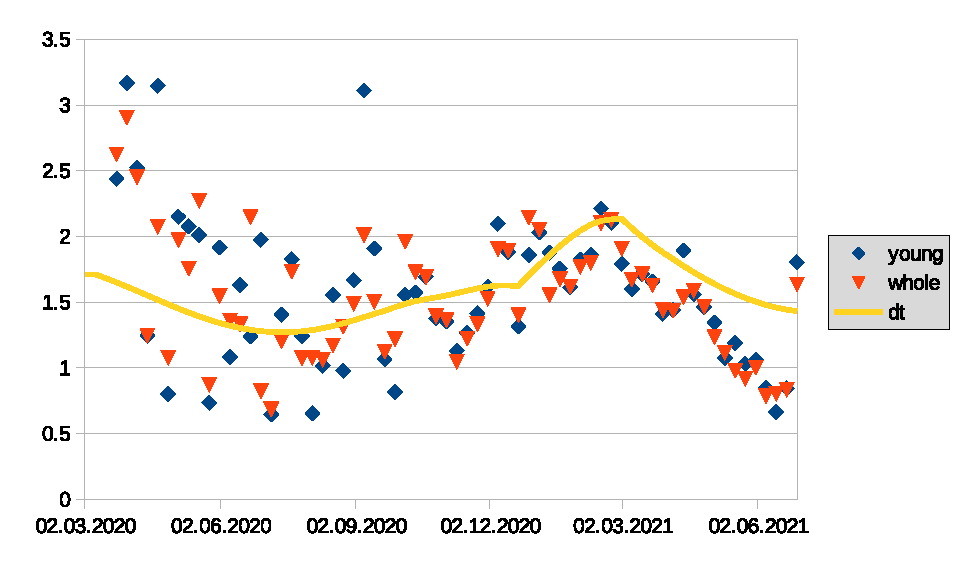
\includegraphics[width=8cm]{dt.eps} 
\caption{Course of $d_t$ (line),  $\frac{Y_{t}}{Y_{t-1} C_{t-2}}$ (triangles) and 
$\frac{\overline{X}_{t}}{\overline{X}_{t-1} C_{t-2}}$ (diamonds) where $overline{X}_{t}=X^k_t+X^f_t+X^s_t+X^e_t$ is the number of infections in all the examined cohorts.
}
\label{fig:dt}
\end{center}
\end{figure}

\begin{table}
\begin{center}
\begin{tabular}{l|cccc} Parameter & Kindergartens & First degree & Second degree & Secondary \\ \hline 
$\alpha$& $0.1^{***}(0.01)$& $0.14^{***}(0.01)$& $0.19^{***}(0.02)$& $0.23^{***}(0.02)$\\
$\beta$& $0.37^{***}(0.01)$& $0.4^{***}(0.01)$& $0.45^{***}(0.01)$& $0.26^{***}(0.02)$\\
$\gamma$& $0.14^{***}(0.01)$& $0.07^{***}(0.01)$& $0.11^{***}(0.01)$& $0.23^{***}(0.01)$\\
\end{tabular}
\caption{Estimation of (\ref{eq:global})}
\label{tab:global}
\end{center}
\end{table}


\section{Covariates}


\begin{center}
\begin{table}
																										TBD										
																		
																						 	\caption{Notes: a -- voluntary, only 15 pupils in a classroom (approx. half), b -- only 4 days from week, c -- only 1st and 2nd classes open, d -- only the last year open, e -- summer vacation, f -- Christmas vacation, g -- autumn vacation,  h -- closed on Wednesday, i -- masks ordered from, j -- different regime among regions according to epidemiological situation, k -- regime change during a week, l -- last year fully open, the rest rotations, m -- starting from Tuesday, valid in all but 3 regions on Monday, n -- open up to decision of directors }										\end{table}															
\end{center}																	 


\section{Detailed Results}

\begin{table}
\begin{center}
\begin{tabular}{lc|cccc} \multicolumn{2}{c}{Model}& Kindergartens & First degree & Second degree & Secondary \\ \hline 
S &$\nu^1$& $0.01^{}(0.03)$&&&\\
($w=15\%$ &$\nu^2$& $-0.01^{}(0.03)$&&&\\
Each)  &$\mu^1$&& $0.15^{***}(0.01)$& $0.19^{***}(0.04)$& $0.16^{***}(0.06)$\\
&$\mu^2$&& $0.29^{***}(0.04)$&& $0.32^{***}(0.08)$\\ 
&$\rho^2$&&& $0.13^{**}(0.05)$&\\ \hline
C &$\mu$&& $0.19^{***}(0.02)$&& $0.2^{***}(0.07)$\\
($w=55\%$) &$\mu-\rho$&&& $0.04^{}(0.05)$&\\ \hline
W &$\nu$& $0^{}(0)$& $0.33^{***}(0.04)$& $0.69^{***}(0.04)$& $0.88^{***}(0.04)$\\
($w=10\%$) &$\mu$&& $0.26^{***}(0.02)$& $0.17^{***}(0.03)$& $0.29^{***}(0.04)$\\
($w=10\%$) &$\rho$&&& $0.11^{***}(0.04)$&\\
&$\rho^\star$&& $0.1^{***}(0.02)$& $0.04^{}(0.03)$&\\
&$\mu^\star$&& $0.11^{***}(0.02)$& $0.13^{***}(0.02)$& $0.21^{***}(0.03)$\\
&$\nu^\star$&& $0.1^{***}(0.03)$& $0.22^{***}(0.03)$& $0.37^{***}(0.03)$\\
&$\gamma$& $0.08^{***}(0.01)$& $-0.16^{***}(0.03)$& $-0.15^{***}(0.03)$& $-0.19^{***}(0.03)$\\ \hline
WH&$\nu$& $-0.01^{***}(0)$& $0.32^{***}(0.04)$& $0.66^{***}(0.04)$& $0.95^{***}(0.04)$\\
($w=5\%$) &$\mu$&& $0.25^{***}(0.02)$& $0.16^{***}(0.03)$& $0.33^{***}(0.04)$\\
&$\rho$&&& $0.1^{**}(0.04)$&\\
&$\rho^\star$&& $0.07^{***}(0.01)$& $0.02^{}(0.03)$&\\
&$\mu^\star$&& $0.07^{***}(0.02)$& $0.12^{***}(0.02)$& $0.19^{***}(0.02)$\\
&$\nu^\star$&& $0.05^{}(0.03)$& $0.19^{***}(0.03)$& $0.43^{***}(0.03)$\\
&$\alpha$& $0.02^{**}(0.01)$& $0.06^{***}(0.02)$& $0.08^{***}(0.03)$& $0.18^{***}(0.03)$\\
&$\beta$& $0.13^{***}(0.01)$& $0.48^{***}(0.02)$& $0.66^{***}(0.03)$& $0.46^{***}(0.03)$\\
&$\gamma$& $0.15^{***}(0.01)$& $-0.05^{**}(0.03)$& $-0.09^{***}(0.03)$& $-0.17^{***}(0.03)$\\
\end{tabular}
\caption{Parameter estimates by individual models.}
\label{tab:params}
\end{center}
\end{table}

\section{Sensitivity Analysis}

\subsection{Natural Immunization}
\label{sa:im}

\begin{tabular}{lc|cccc} \multicolumn{2}{c}{Model}& Kindergartens & First degree & Second degree & Secondary \\ \hline 
S &$\nu^1$& $0^{}(0.03)$&&&\\
($w=15\%$ &$\nu^2$& $-0.01^{}(0.03)$&&&\\
Each)  &$\mu^1$&& $0.16^{***}(0.02)$& $0.19^{***}(0.04)$& $0.16^{***}(0.06)$\\
&$\mu^2$&& $0.3^{***}(0.04)$&& $0.33^{***}(0.08)$\\ 
&$\rho^2$&&& $0.14^{**}(0.06)$&\\ \hline
C &$\mu$&& $0.2^{***}(0.02)$&& $0.19^{***}(0.07)$\\
($w=55\%$) &$\mu-\rho$&&& $0.04^{}(0.05)$&\\ \hline
W &$\nu$& $0^{}(0)$& $0.26^{***}(0.04)$& $0.64^{***}(0.04)$& $0.88^{***}(0.04)$\\
($w=10\%$) &$\mu$&& $0.23^{***}(0.02)$& $0.12^{***}(0.03)$& $0.28^{***}(0.04)$\\
($w=10\%$) &$\rho$&&& $0.1^{**}(0.04)$&\\
&$\rho^\star$&& $0.12^{***}(0.02)$& $0.05^{*}(0.03)$&\\
&$\mu^\star$&& $0.13^{***}(0.02)$& $0.14^{***}(0.02)$& $0.26^{***}(0.03)$\\
&$\nu^\star$&& $0.03^{}(0.04)$& $0.17^{***}(0.04)$& $0.36^{***}(0.05)$\\
&$\gamma$& $0.09^{***}(0.01)$& $-0.13^{***}(0.03)$& $-0.11^{***}(0.03)$& $-0.22^{***}(0.03)$\\ \hline
WH&$\nu$& $-0.01^{***}(0)$& $0.26^{***}(0.04)$& $0.61^{***}(0.03)$& $0.92^{***}(0.04)$\\
($w=5\%$) &$\mu$&& $0.23^{***}(0.02)$& $0.11^{***}(0.03)$& $0.3^{***}(0.04)$\\
&$\rho$&&& $0.09^{**}(0.04)$&\\
&$\rho^\star$&& $0.08^{***}(0.02)$& $0.02^{}(0.03)$&\\
&$\mu^\star$&& $0.08^{***}(0.02)$& $0.13^{***}(0.02)$& $0.22^{***}(0.03)$\\
&$\nu^\star$&& $-0.04^{}(0.04)$& $0.13^{***}(0.03)$& $0.38^{***}(0.04)$\\
&$\alpha$& $0.02^{*}(0.01)$& $0.08^{***}(0.02)$& $0.11^{***}(0.03)$& $0.22^{***}(0.03)$\\
&$\beta$& $0.14^{***}(0.01)$& $0.5^{***}(0.02)$& $0.66^{***}(0.03)$& $0.49^{***}(0.03)$\\
&$\gamma$& $0.16^{***}(0.01)$& $-0.02^{}(0.02)$& $-0.04^{*}(0.02)$& $-0.17^{***}(0.03)$\\
\end{tabular}

\begin{tabular}{l|cc|cc|cc} & \multicolumn{2}{c}{First degree} & \multicolumn{2}{c}{Second degree} & \multicolumn{2}{c}{Secondary} \\ Parameter  & par. & rel. & par. & rel.& par. & rel.\\  \hline  
$\nu$& $0.26(0.04)$&$0.15$& $0.63(0.04)$&$0.15$& $0.9(0.04)$& $0.15$\\
$\mu$& $0.21(0.02)$&$1$& $0.15(0.04)$&$0.3$& $0.22(0.06)$& $1$\\
$\rho$&&& $0.12(0.05)$&$0.3$&& \\
$\rho^\star$& $0.1(0.02)$&$0.15$& $0.04(0.03)$&$0.15$&& \\
$\mu^\star$& $0.11(0.02)$&$0.15$& $0.13(0.02)$&$0.15$& $0.25(0.03)$& $0.15$\\
$\nu^\star$& $0.01(0.04)$&$0.15$& $0.16(0.03)$&$0.15$& $0.37(0.05)$& $0.15$\\
$\gamma$& $-0.02(0.02)$& –& $-0.04(0.02)$& –& $-0.17(0.03)$& –\\
$\nu$& $0.58(0.04)$& –& $0.76(0.06)$& –& $0.7(0.06)$& –\\
\end{tabular}



tmp

\begin{tabular}{lc|cccc} \multicolumn{2}{c}{Model}& Kindergartens & First degree & Second degree & Secondary \\ \hline 
S &$\nu^1$& $0.01^{}(0.04)$&&&\\
($w=15\%$ &$\nu^2$& $-0.01^{}(0.04)$&&&\\
Each)  &$\mu^1$&& $0.19^{***}(0.02)$& $0.2^{***}(0.04)$& $0.17^{***}(0.06)$\\
&$\mu^2$&& $0.32^{***}(0.04)$&& $0.34^{***}(0.08)$\\ 
&$\rho^2$&&& $0.14^{**}(0.06)$&\\ \hline
C &$\mu$&& $0.23^{***}(0.02)$&& $0.2^{***}(0.07)$\\
($w=55\%$) &$\mu-\rho$&&& $0.04^{}(0.06)$&\\ \hline
W &$\nu$& $0^{}(0)$& $0.12^{***}(0.04)$& $0.53^{***}(0.04)$& $0.78^{***}(0.04)$\\
($w=10\%$) &$\mu$&& $0.16^{***}(0.03)$& $0.02^{}(0.03)$& $0.18^{***}(0.04)$\\
($w=10\%$) &$\rho$&&& $0.08^{*}(0.05)$&\\
&$\rho^\star$&& $0.13^{***}(0.02)$& $0.06^{*}(0.04)$&\\
&$\mu^\star$&& $0.12^{***}(0.03)$& $0.15^{***}(0.03)$& $0.32^{***}(0.04)$\\
&$\nu^\star$&& $0.09^{*}(0.04)$& $0.25^{***}(0.04)$& $0.56^{***}(0.05)$\\
&$\gamma$& $0.11^{***}(0.01)$& $-0.05^{*}(0.03)$& $-0.05^{*}(0.03)$& $-0.18^{***}(0.03)$\\ \hline
WH&$\nu$& $-0.01^{**}(0)$& $0.15^{***}(0.04)$& $0.53^{***}(0.04)$& $0.87^{***}(0.03)$\\
($w=5\%$) &$\mu$&& $0.18^{***}(0.03)$& $0.03^{}(0.03)$& $0.23^{***}(0.03)$\\
&$\rho$&&& $0.06^{}(0.05)$&\\
&$\rho^\star$&& $0.09^{***}(0.02)$& $0.05^{}(0.04)$&\\
&$\mu^\star$&& $0.07^{***}(0.02)$& $0.15^{***}(0.02)$& $0.28^{***}(0.03)$\\
&$\nu^\star$&& $0.01^{}(0.04)$& $0.22^{***}(0.04)$& $0.61^{***}(0.04)$\\
&$\alpha$& $0.02^{*}(0.01)$& $0.1^{***}(0.02)$& $0.12^{***}(0.03)$& $0.25^{***}(0.03)$\\
&$\beta$& $0.16^{***}(0.01)$& $0.52^{***}(0.03)$& $0.71^{***}(0.04)$& $0.55^{***}(0.04)$\\
&$\gamma$& $0.17^{***}(0.01)$& $0.04^{*}(0.02)$& $0^{}(0.02)$& $-0.15^{***}(0.03)$\\
\end{tabular}
\begin{tabular}{l|cccc} Parameter & Kindergartens & First degree & Second degree & Secondary \\ \hline 
$\alpha$& $0.14^{***}(0.01)$& $0.2^{***}(0.01)$& $0.28^{***}(0.02)$& $0.33^{***}(0.02)$\\
$\beta$& $0.36^{***}(0.01)$& $0.38^{***}(0.01)$& $0.44^{***}(0.02)$& $0.29^{***}(0.02)$\\
$\gamma$& $0.18^{***}(0.01)$& $0.13^{***}(0.01)$& $0.14^{***}(0.01)$& $0.21^{***}(0.01)$\\
\end{tabular}

\begin{tabular}{l|ccc|ccc|ccc} Para- & \multicolumn{3}{c}{First degree} & \multicolumn{3}{c}{Second degree} & \multicolumn{3}{c}{Secondary} \\ meter  & par. & inc. & rel. & par. & inc.& rel.& par.& inc. & rel.\\  \hline  
$\nu$& $0.13(0.04)$& $0.2$&$0.15$& $0.53(0.04)$& $0.64$&$0.15$& $0.81(0.04)$& $1.24$& $0.15$\\
$\mu$& $0.23(0.02)$& $0.35$&$1$& $0.11(0.04)$& $0.13$&$0.3$& $0.21(0.07)$& $0.33$& $1$\\
$\rho$&&&& $0.11(0.05)$& $0.13$&$0.3$&&& \\
$\rho^\star$& $0.12(0.02)$& $0.18$&$0.15$& $0.06(0.04)$& $0.07$&$0.15$&&& \\
$\mu^\star$& $0.1(0.03)$& $0.15$&$0.15$& $0.15(0.03)$& $0.18$&$0.15$& $0.31(0.04)$& $0.47$& $0.15$\\
$\nu^\star$& $0.06(0.04)$& $0.09$&$0.15$& $0.24(0.04)$& $0.29$&$0.15$& $0.58(0.05)$& $0.88$& $0.15$\\
$\gamma$& $0.04(0.02)$& –& –& $0(0.02)$& –& –& $-0.15(0.03)$& –& –\\
$\omega$& $0.62(0.05)$& –& –& $0.83(0.07)$& –& –& $0.81(0.07)$& –& –\\
\end{tabular}


\end{document}
